\documentclass[portuguese]{beamer}

\usetheme{moloch}

\title{Ofuscação de código em arquivos ELF utilizando relocação}
\author{João C. Fukuda}
\institute{Cryptorave}
\date{2026}

\begin{filecontents}{\jobname.bib}
@online{netspooky,
	author = {Netspooky},
	title = {ELF Binary Mangling Series},
	url = {https://n0.lol/ebm/}
}

@online{sblip,
	author = {sblip},
	title = {Implementing the PT\_NOTE Infection Method in x64 Assembly},
	url = {https://tmpout.sh/1/2.html}
}

@online{s01den,
	author = {s01den},
	title = {A short note on entrypoint obscuring in ELF binaries},
	url = {https://tmpout.sh/2/2.html}
}

@online{s0s4,
	author = {S0S4},
	title = {Relocation Revelation: Unpacking the Secrets of ELF},
	url = {https://tmpout.sh/4/4.html}
}

@online{elf.h,
	author = {GNU C Library master sources},
	title = {sourceware.org Git - glibc.git/blob - elf/elf.h},
	url = {https://sourceware.org/git/?p=glibc.git;a=blob;f=elf/elf.h;h=46a01281cb0fb5322d5124f0443c11dea4d5b721;hb=f762ccf84f122d1354f103a151cba8bde797d521}
}

@online{relobfuscate,
	author = {peding},
	title = {relobfuscate},
	url = {https://github.com/peding/relobfuscate}
}

@online{elf-rela-obfuscation,
	author = {ulexec},
	title = {elf\_rela\_obfuscation},
	url = {https://github.com/ulexec/elf\_rela\_obfuscation}
}
\end{filecontents}

\usepackage{gruvbox}
\usepackage{minted}
\usepackage[provide=*]{babel}
\usepackage[backend=bibtex,style=numeric-comp,sorting=none]{biblatex}

\addbibresource{\jobname.bib}

\begin{document}

\frame{\titlepage}

\begin{frame}
	\frametitle{Quem sou eu?}
	\framesubtitle{whoami}
	\begin{itemize}
		\item Bacharel em Sistemas de Informação
		\item Membro fundador do Each inTheShell\_
		\item Migrando de Backend para Cibersegurança
		\item Apreciador do baixo nível
	\end{itemize}
\end{frame}

\begin{frame}
	\frametitle{Conteúdo}
	\framesubtitle{head}
	\begin{itemize}
		\item Motivação
		\item ELF Refresher
		\item A Ideia
		\item Desenvolvimento
		\item Problemas e Limitações
		\item Detecção
	\end{itemize}
\end{frame}

\begin{frame}
	\frametitle{Motivação}
	\framesubtitle{hostname}
	\begin{itemize}
		\item Inspirações:
		\begin{itemize}
			\item Netspooky's ELF Binary Mangling Series\cite{netspooky}
			\item sblip's Implementing the PT\_NOTE Infection Method In x64 Assembly\cite{sblip}
			\item s01den's A short note on entrypoint obscuring in ELF binaries\cite{s01den}
			\item S0S4's Relocation Revelation: Unpacking the Secrets of ELF\cite{s0s4}
		\end{itemize}
		\item Curiosidade \& Conhecimento
	\end{itemize}
\end{frame}

\begin{frame}
	\frametitle{Quick ELF Refresher}
	\framesubtitle{info}
	\begin{itemize}
		\item A estrutura de um arquivo ELF\cite{elf.h}
		\begin{itemize}
			\item Elf Header (\texttt{Elf64\_Ehdr})
			\begin{itemize}
				\item \texttt{e\_type}, \texttt{e\_entry}
				\item \texttt{e\_phoff}, \texttt{e\_phentsize}, \texttt{e\_phnum}
				\item \texttt{e\_shoff}, \texttt{e\_shentsize}, \texttt{e\_shnum}
			\end{itemize}
			\item Program Header (\texttt{Elf64\_Phdr})
			\begin{itemize}
				\item Loadable program segment (\texttt{PT\_LOAD})
			\end{itemize}
			\item Section Header (\texttt{Elf64\_Shdr})
			\begin{itemize}
				\item Relocation entries with addends (\texttt{SHT\_RELA})
				\item Relocation entries, no addends (\texttt{SHT\_REL})
			\end{itemize}
		\end{itemize}
	\end{itemize}
\end{frame}

\begin{frame}
	\frametitle{A Ideia}
	\framesubtitle{cat}
	\begin{itemize}
		\item \textbf{Cenário:} Construir um arquivo ELF do zero
		\begin{itemize}
			\item começar com um arquivo ELF simples e funcional
		\end{itemize}
		\item \textbf{Objetivo:} Fazer a relocação dinâmica funcionar
		\begin{itemize}
			\item iterar sobre o arquivo até obter algum resultado
		\end{itemize}
		\item \textbf{Conclusão:} Esconder um código na sessão de relocação
		\begin{itemize}
			\item fazer rodar outro código do que está presente no segmento PT\_LOAD
		\end{itemize}
	\end{itemize}
\end{frame}

\begin{frame}[plain]
	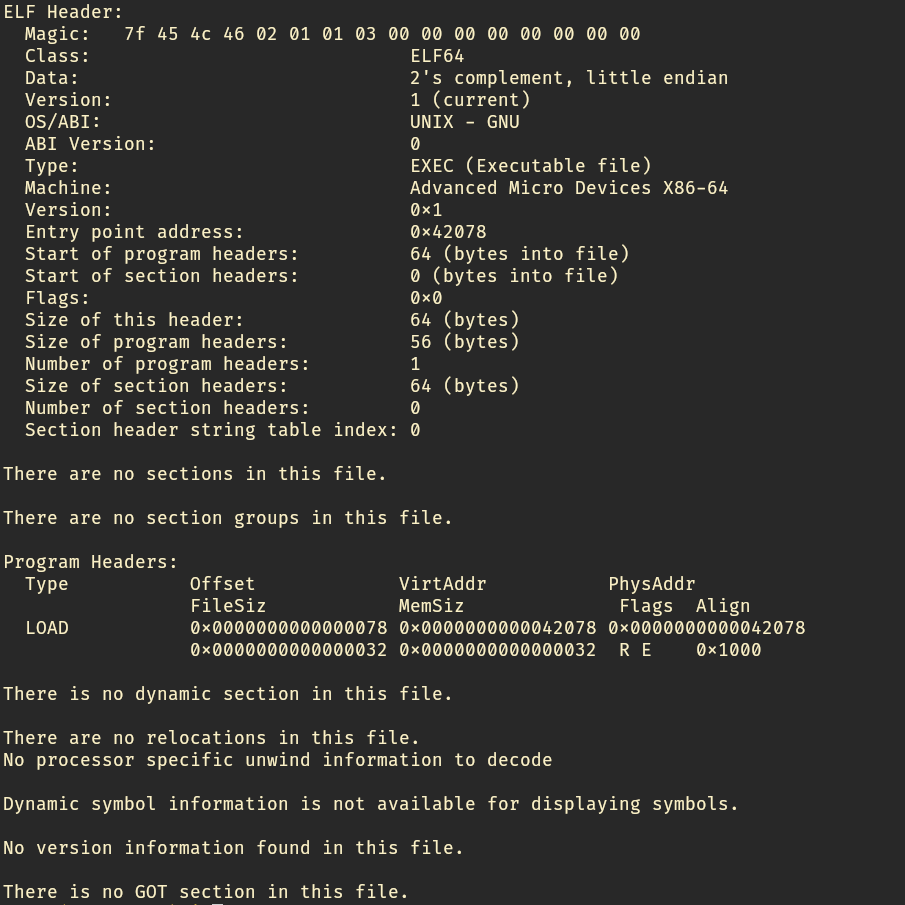
\includegraphics[height=\textheight]{img/0-readelf.png}
\end{frame}

\begin{frame}[plain]
	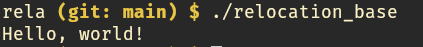
\includegraphics[width=\textwidth]{img/0-exec.png}
\end{frame}

\begin{frame}[plain]
	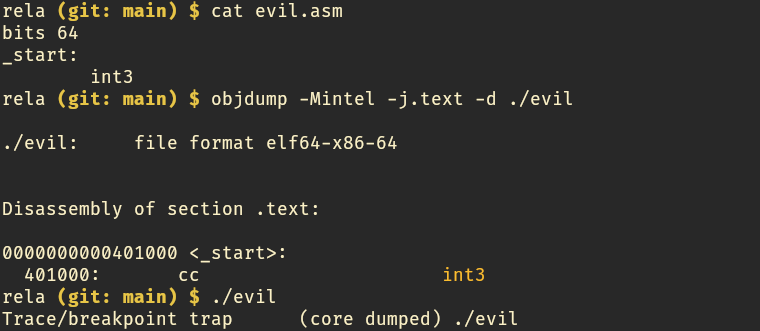
\includegraphics[width=\textwidth]{img/0-evil.png}
\end{frame}

\section{Construindo um ELF do zero}

\begin{frame}[plain]
	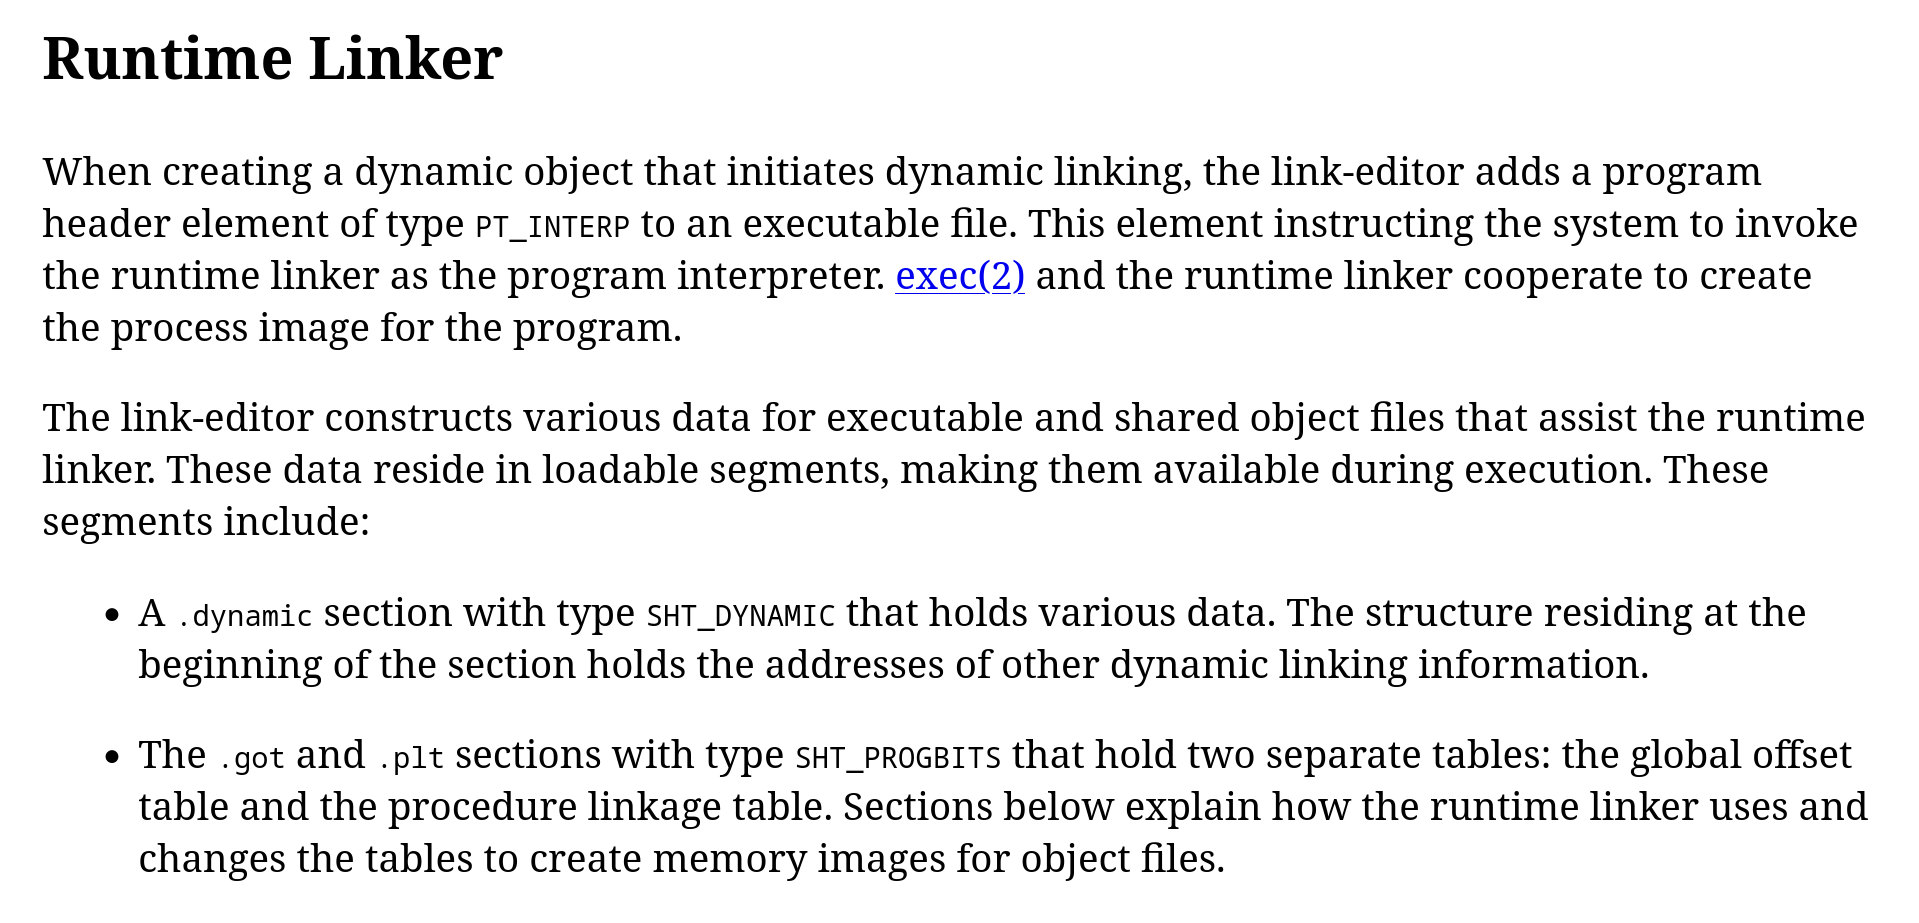
\includegraphics[width=\textwidth]{img/0-linker_doc.png}
\end{frame}

\begin{frame}[plain]
	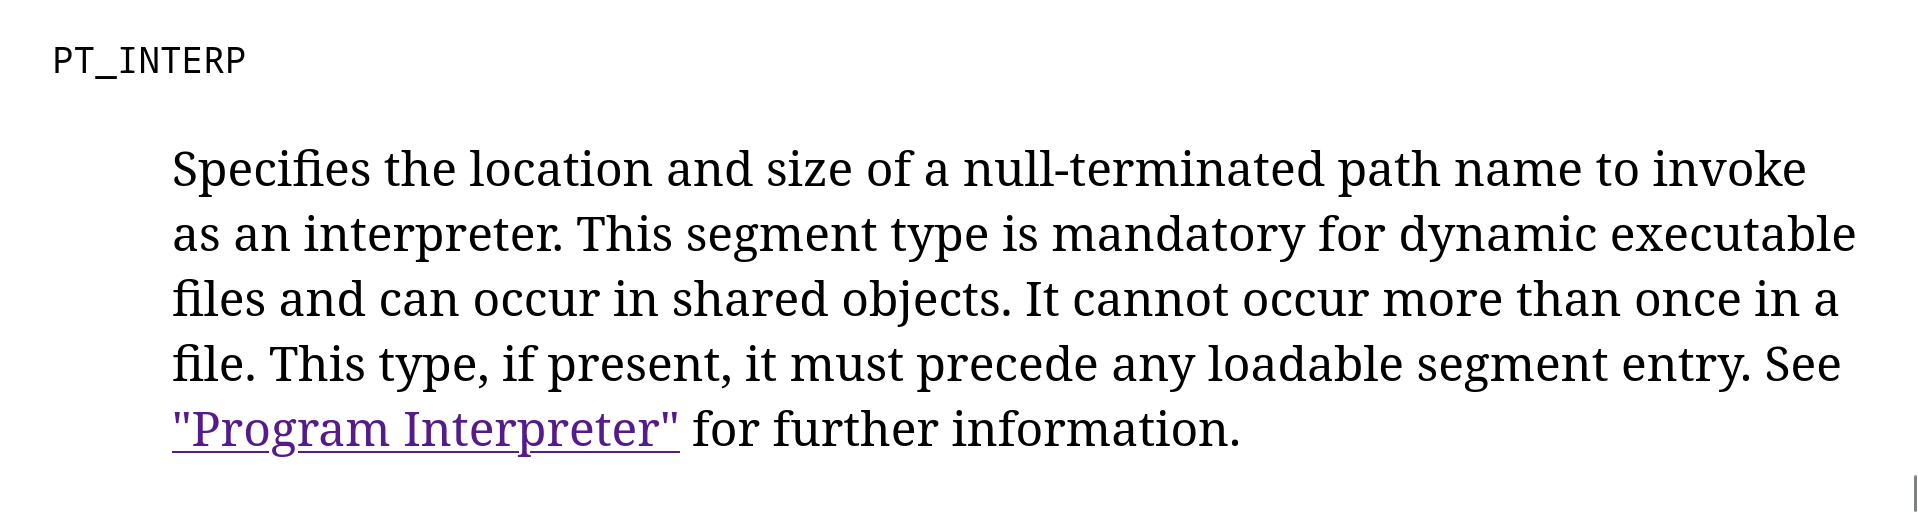
\includegraphics[width=\textwidth]{img/0-interp_doc.png}
\end{frame}

\begin{frame}[plain]
	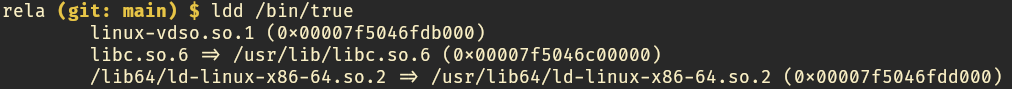
\includegraphics[width=\textwidth]{img/0-ldd.png}
\end{frame}

\begin{frame}
	\frametitle{Construindo do Zero}
	\framesubtitle{code}
	\begin{itemize}
		\item modificar o tipo do arquivo de \texttt{ET\_EXEC} para \texttt{ET\_DYN}
		\item adicionar o segmento \texttt{PT\_INTERP}
		\item adicionar a sessão \texttt{SHT\_RELA}
	\end{itemize}
\end{frame}

\begin{frame}[plain]
	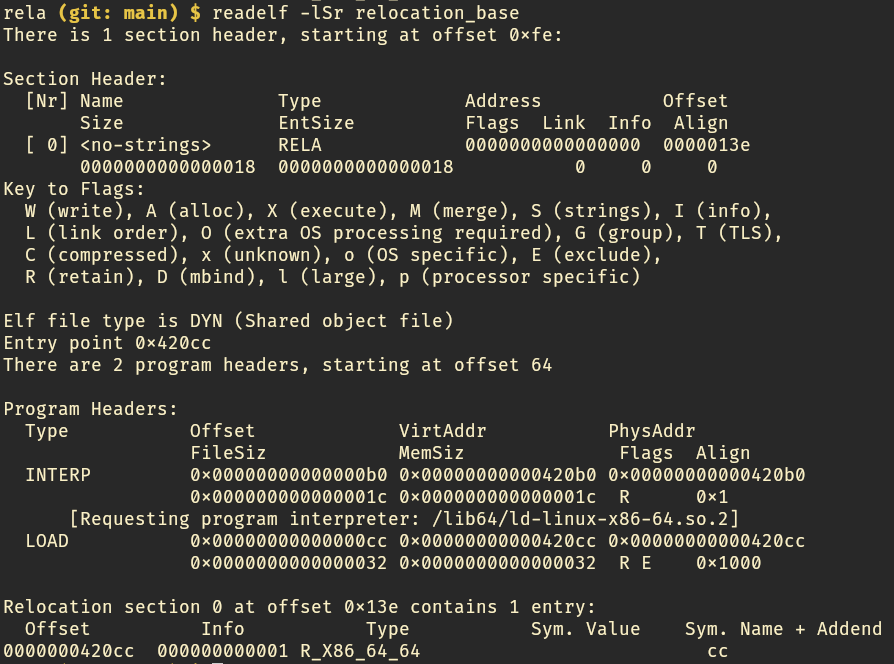
\includegraphics[width=\textwidth]{img/1-readelf.png}
\end{frame}

\begin{frame}[plain]
	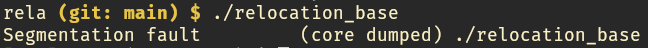
\includegraphics[width=\textwidth]{img/1-exec.png}
\end{frame}

\begin{frame}[plain]
	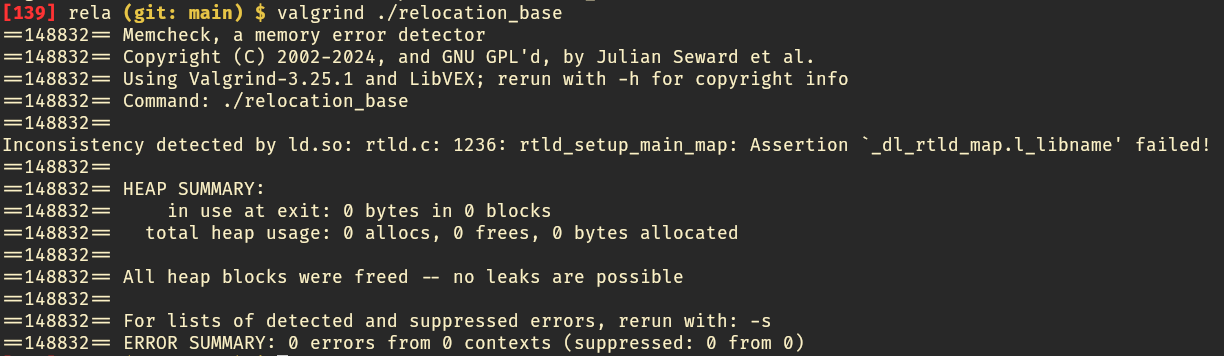
\includegraphics[width=\textwidth]{img/1-valgrind.png}
\end{frame}

\begin{frame}[plain]
	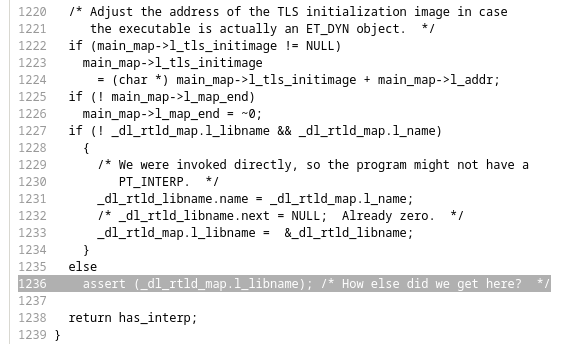
\includegraphics[width=\textwidth]{img/1-assert_source.png}
\end{frame}

\begin{frame}[plain]
	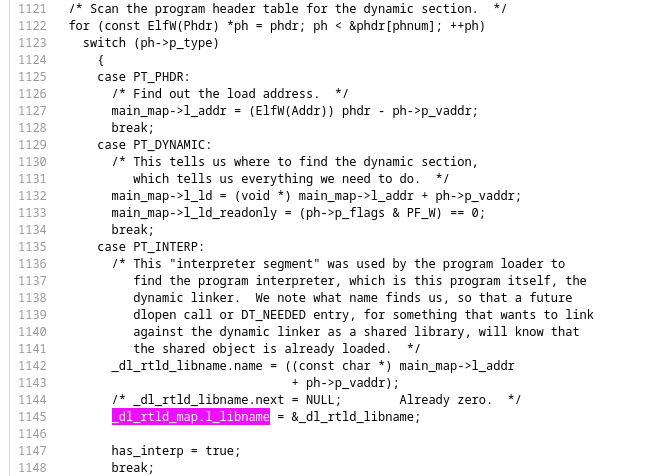
\includegraphics[width=\textwidth]{img/1-cause_source.png}
\end{frame}

\begin{frame}[plain]
	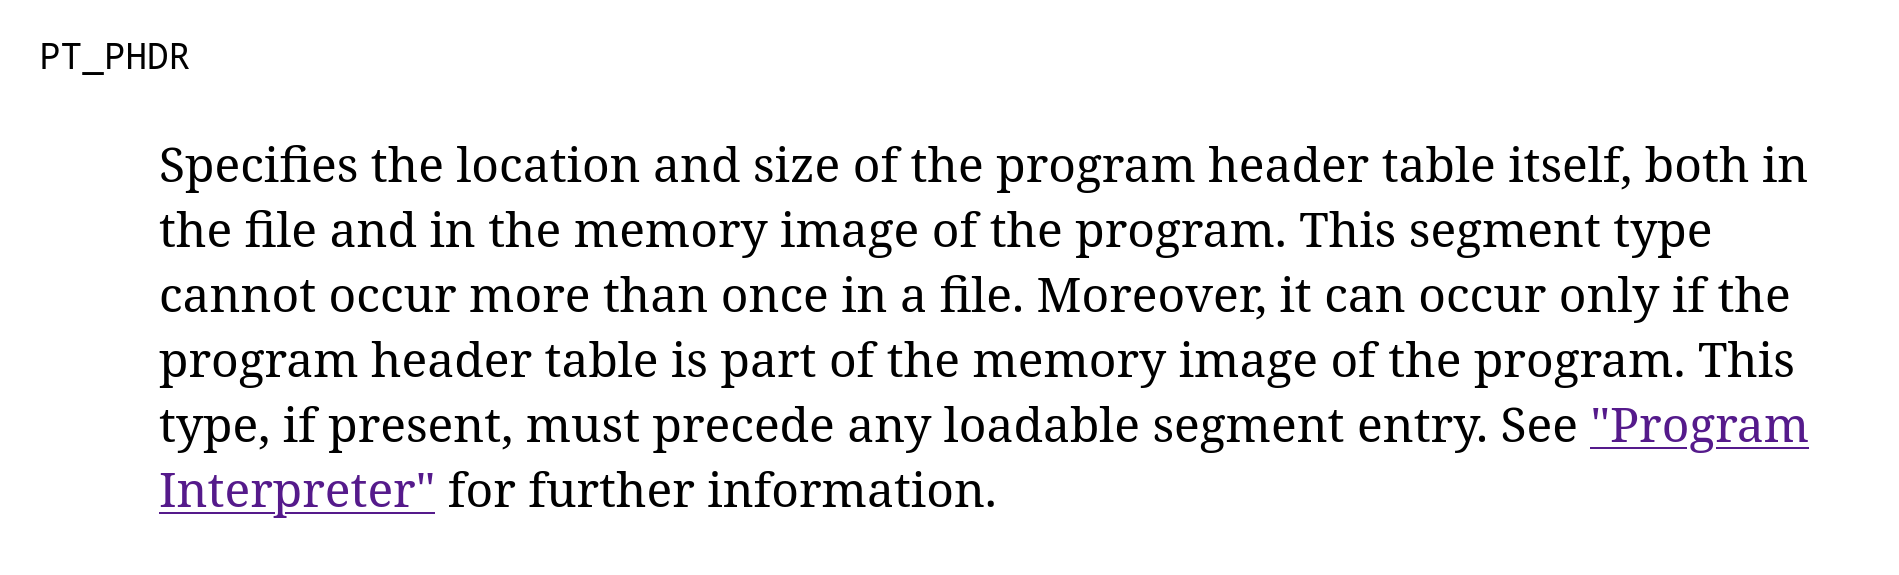
\includegraphics[width=\textwidth]{img/1-phdr_doc.png}
\end{frame}

\begin{frame}
	\frametitle{Construindo do Zero}
	\framesubtitle{code}
	\begin{itemize}
		\item adicionar o segmento \texttt{PT\_PHDR}
		\item modificar o alcance do segmento \texttt{PT\_LOAD} para encorporar os \texttt{Phdrs}
	\end{itemize}
\end{frame}

\begin{frame}[plain]
	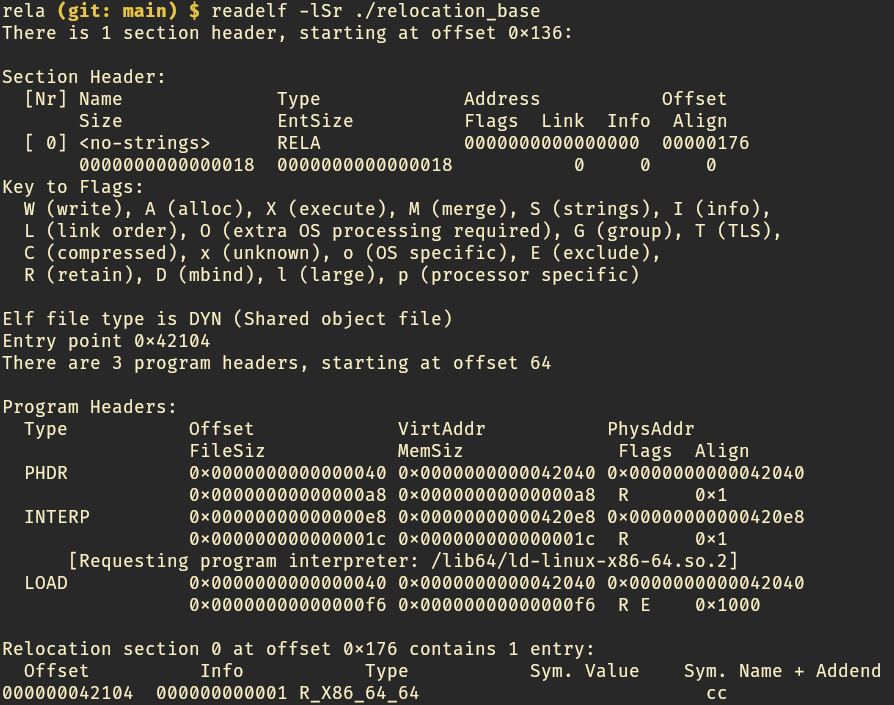
\includegraphics[width=\textwidth]{img/2-readelf.png}
\end{frame}

\begin{frame}[plain]
	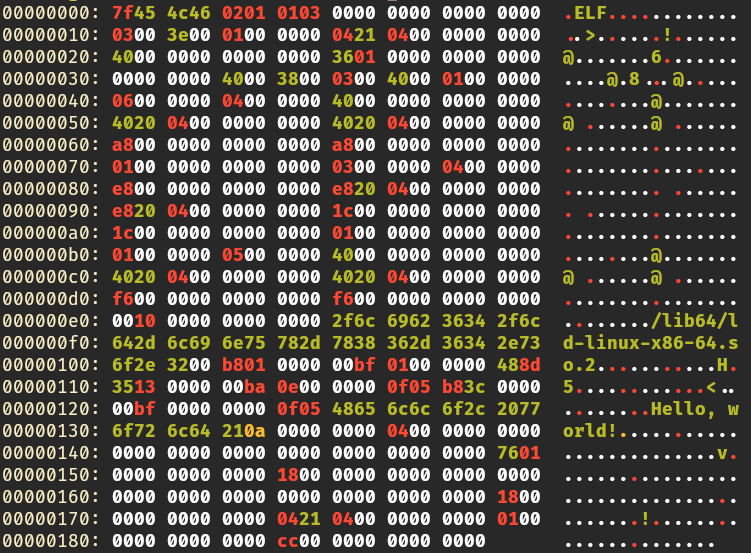
\includegraphics[width=\textwidth]{img/2-hexdump.png}
\end{frame}

\begin{frame}[plain]
	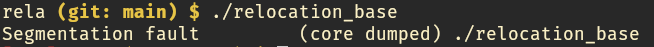
\includegraphics[width=\textwidth]{img/2-exec.png}
\end{frame}

\begin{frame}[plain]
	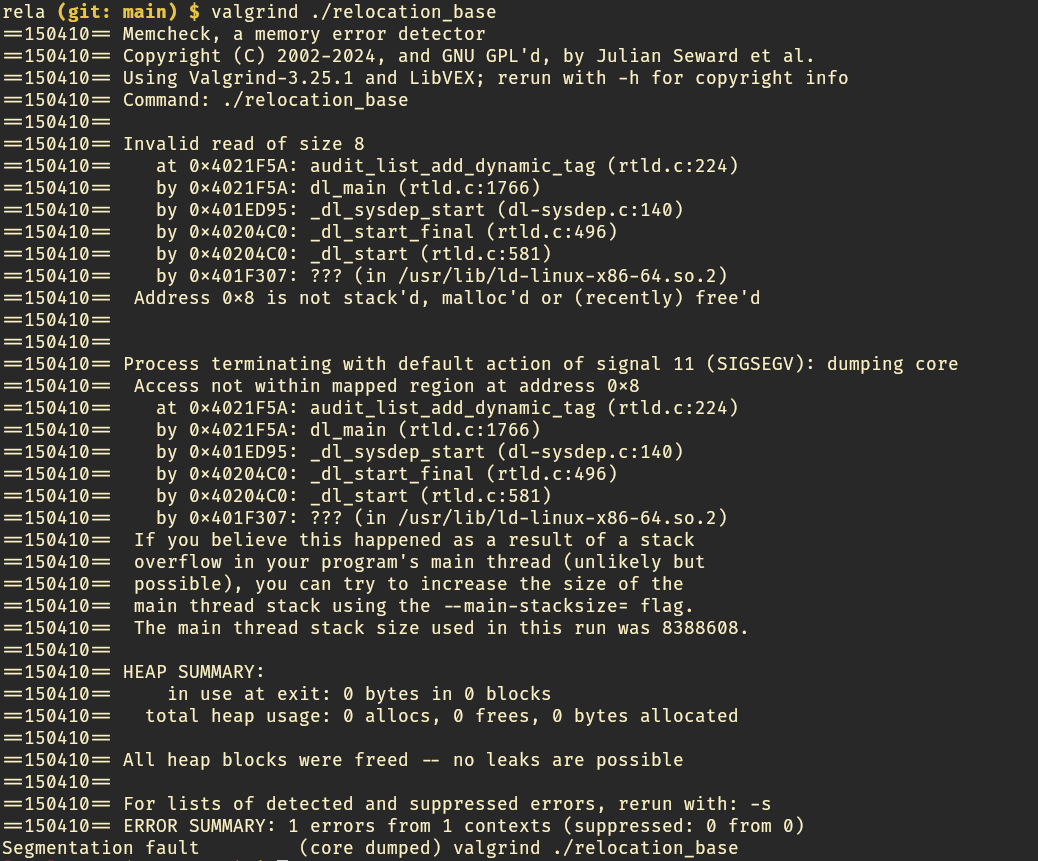
\includegraphics[width=\textwidth]{img/2-valgrind.png}
\end{frame}

\begin{frame}[plain]
	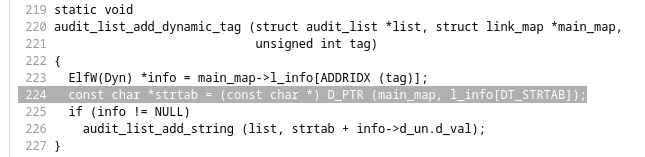
\includegraphics[width=\textwidth]{img/2-cause_source.png}
\end{frame}

\begin{frame}[plain]
	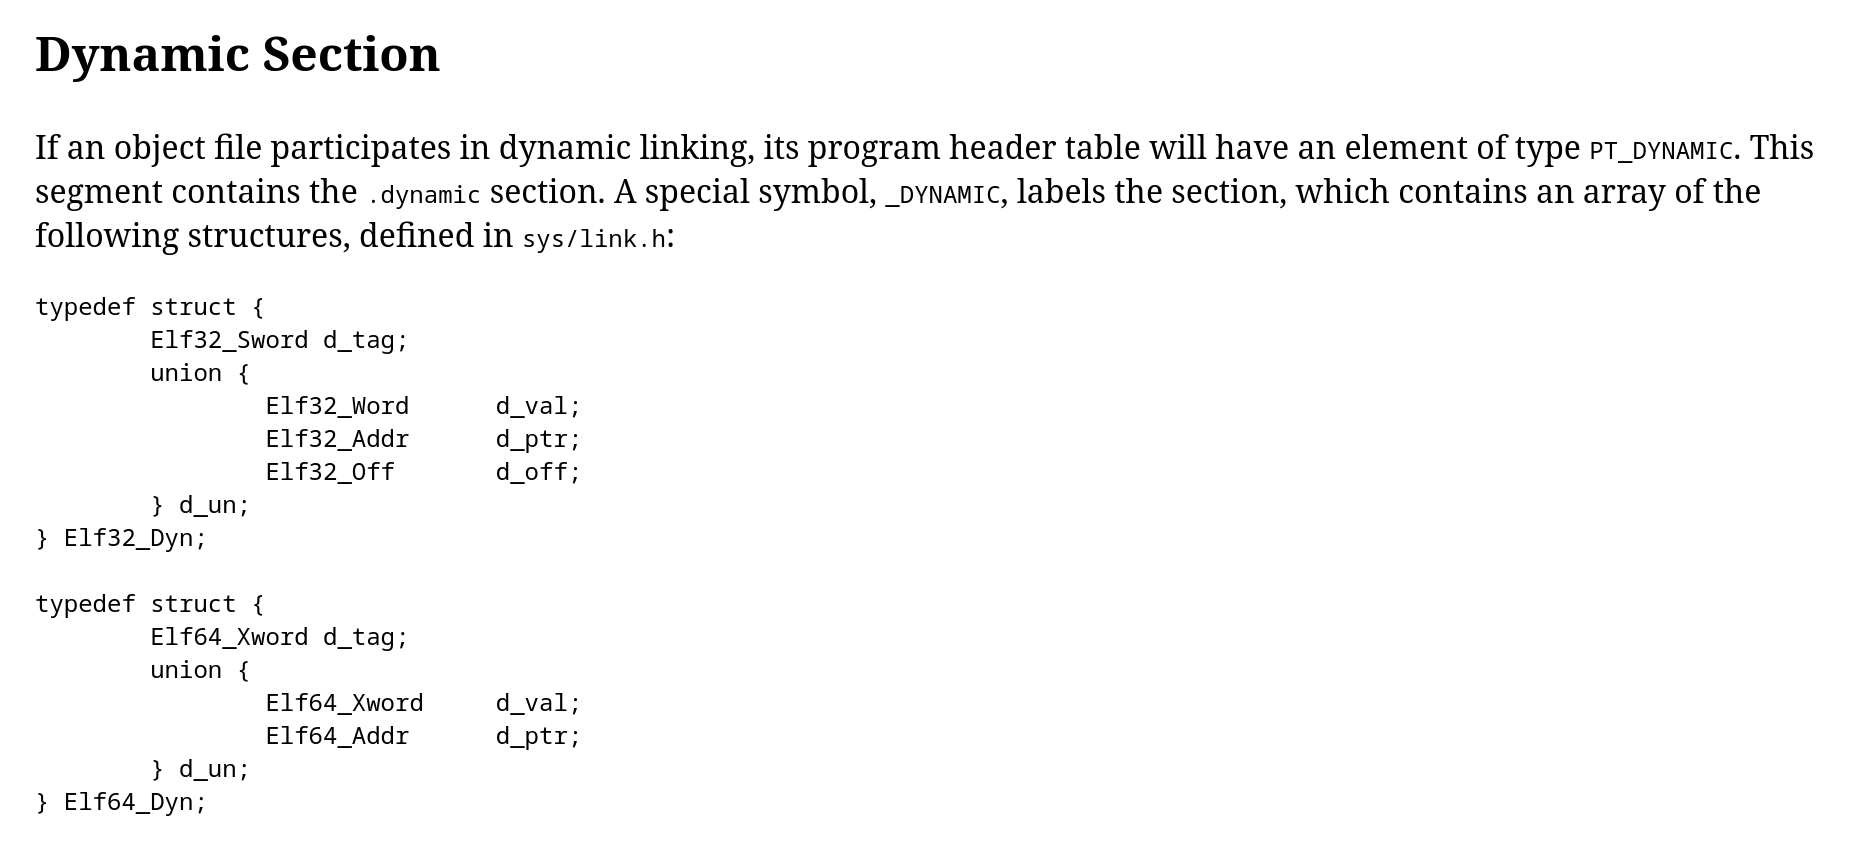
\includegraphics[width=\textwidth]{img/2-dynamic_doc.png}
\end{frame}

\begin{frame}[plain]
	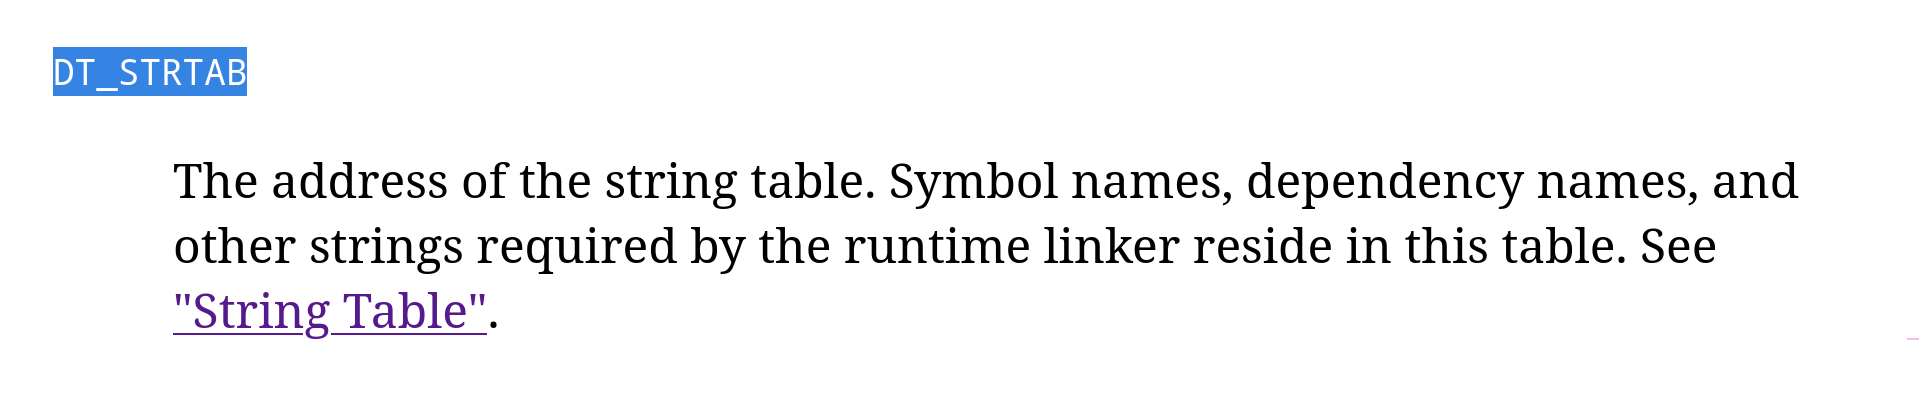
\includegraphics[width=\textwidth]{img/2-DT_STRTAB_doc.png}
\end{frame}

\begin{frame}[plain]
	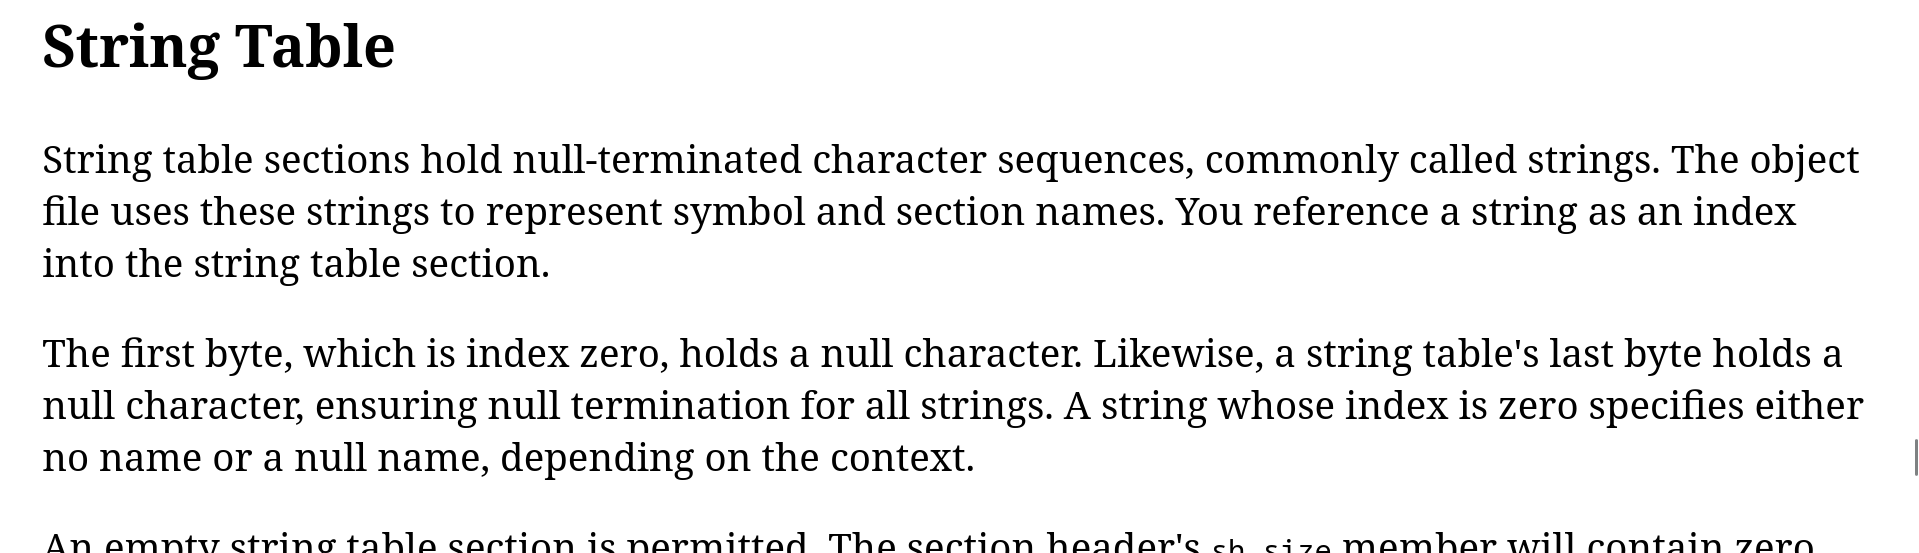
\includegraphics[width=\textwidth]{img/2-strtab_doc.png}
\end{frame}

\begin{frame}
	\frametitle{Construindo do Zero}
	\framesubtitle{code}
	\begin{itemize}
		\item adicionar a sessão \texttt{SHT\_STRTAB}
		\item adicionar o segmento \texttt{PT\_DYNAMIC}
		\begin{itemize}
			\item adicionar a tag dinâmica \texttt{DT\_STRTAB}
		\end{itemize}
	\end{itemize}
\end{frame}

\begin{frame}[plain]
	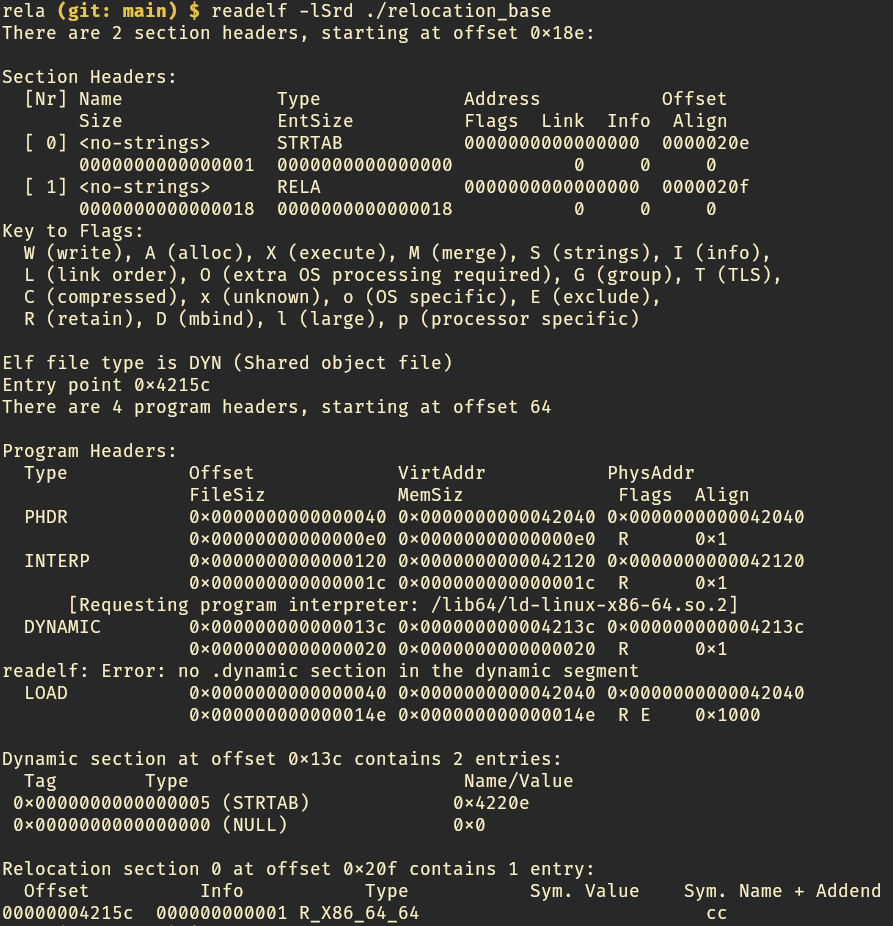
\includegraphics[height=\textheight]{img/3-readelf.png}
\end{frame}

\begin{frame}[plain]
	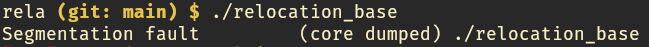
\includegraphics[width=\textwidth]{img/3-exec.png}
\end{frame}

\begin{frame}[plain]
	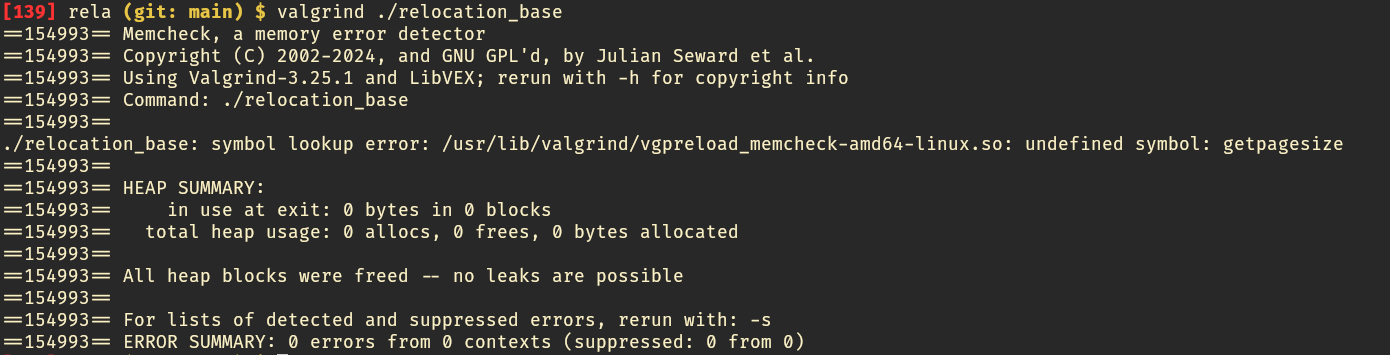
\includegraphics[width=\textwidth]{img/3-valgrind.png}
\end{frame}

\begin{frame}[plain]
	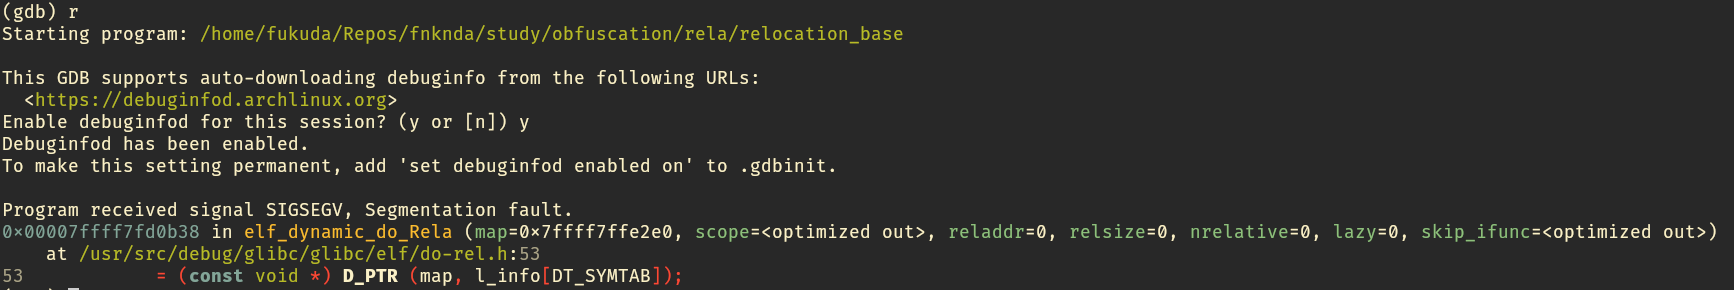
\includegraphics[width=\textwidth]{img/3-gdb.png}
\end{frame}

\begin{frame}[plain]
	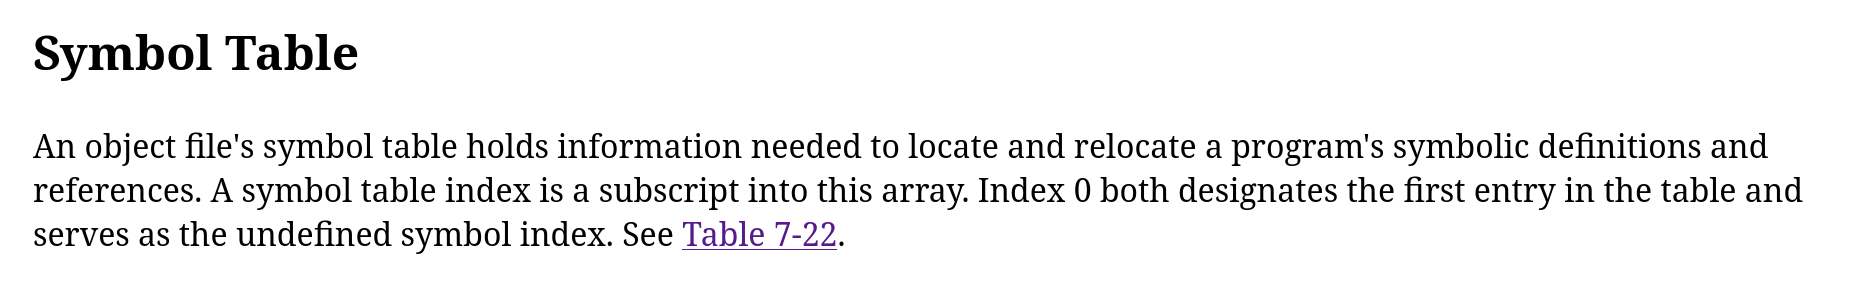
\includegraphics[width=\textwidth]{img/3-symtab_doc.png}
\end{frame}

\begin{frame}[plain]
	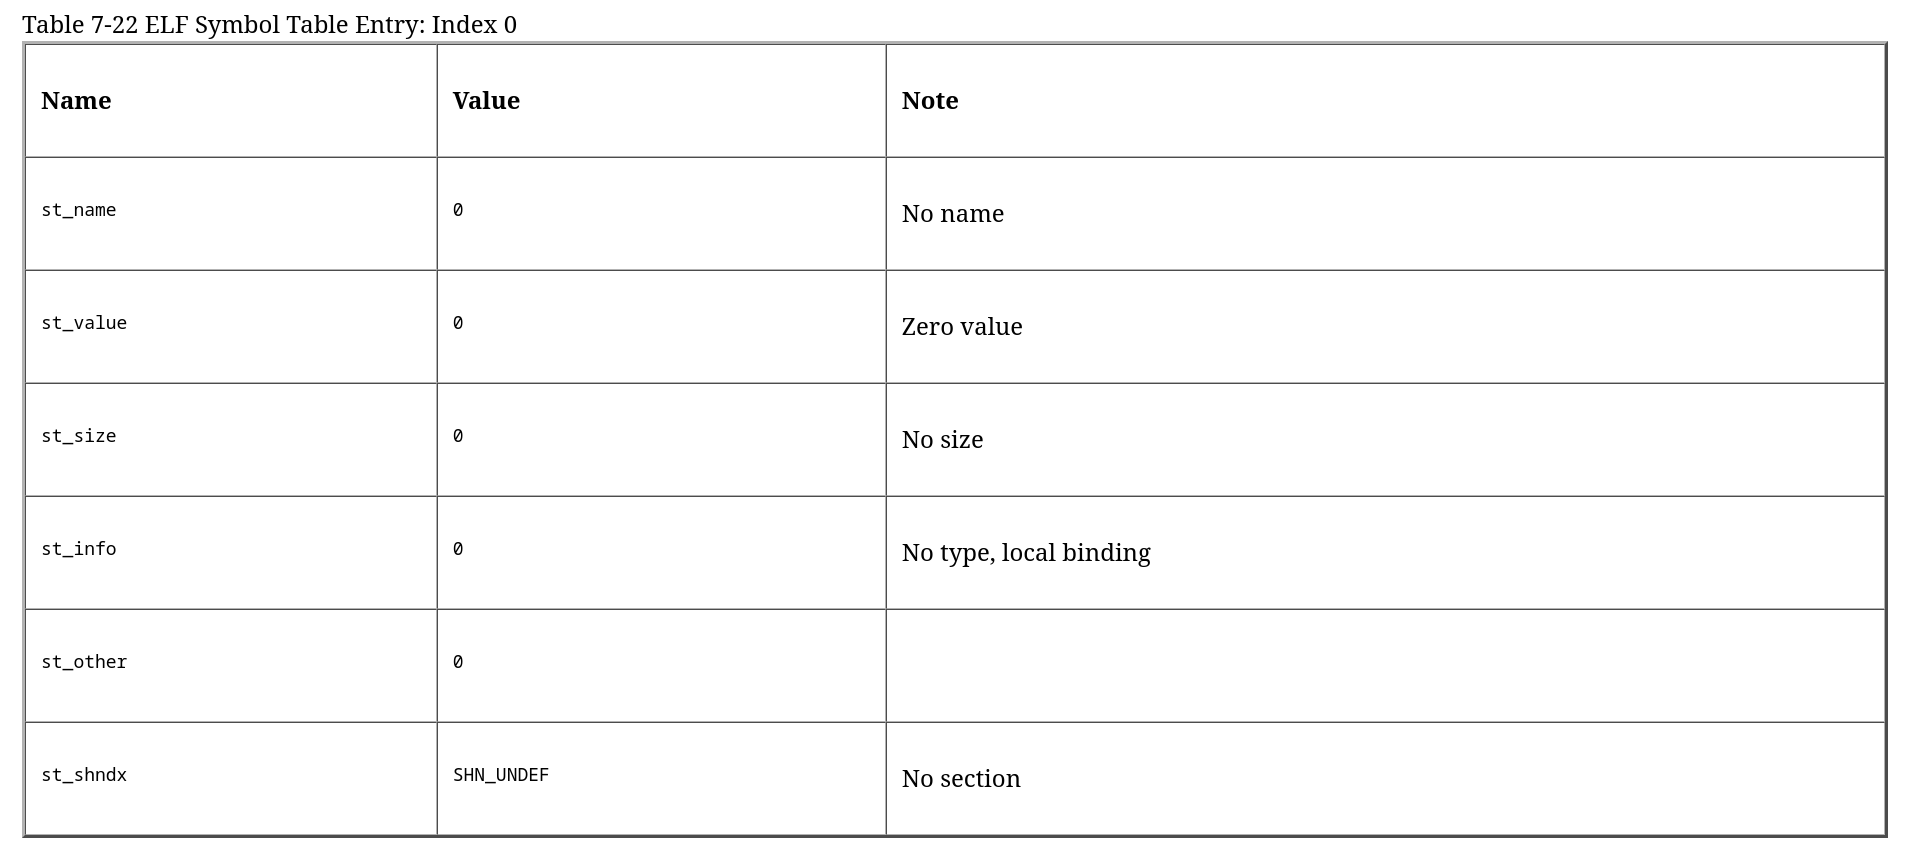
\includegraphics[width=\textwidth]{img/3-index0_doc.png}
\end{frame}

\begin{frame}
	\frametitle{Construindo do Zero}
	\framesubtitle{code}
	\begin{itemize}
		\item adicionar a sessão \texttt{SHT\_SYMTAB}
		\item adicionar a tag dinâmica \texttt{DT\_SYMTAB}
	\end{itemize}
\end{frame}

\begin{frame}[plain]
	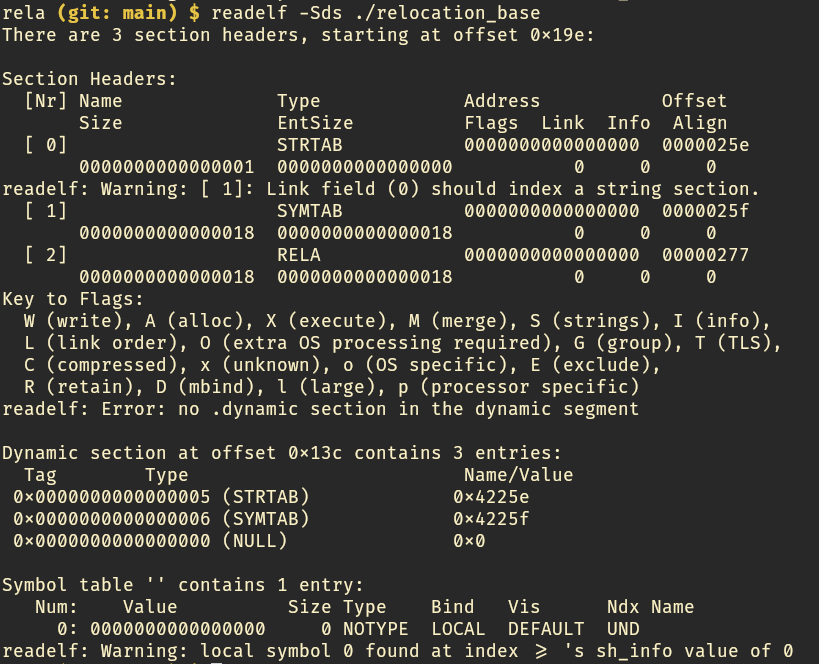
\includegraphics[height=\textheight]{img/4-readelf.png}
\end{frame}

\begin{frame}[plain]
	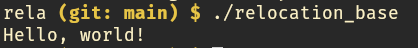
\includegraphics[width=\textwidth]{img/4-exec.png}
\end{frame}

\begin{frame}[plain]
	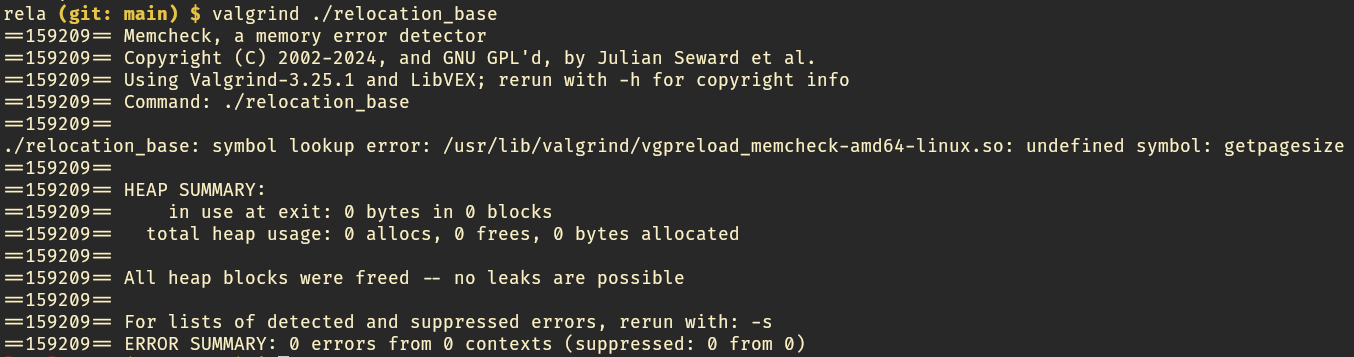
\includegraphics[width=\textwidth]{img/4-valgrind.png}
\end{frame}

\begin{frame}
	\frametitle{Construindo do Zero}
	\framesubtitle{code}
	\begin{itemize}
		\item arrumar as tags dinâmicas até rodar
	\end{itemize}
\end{frame}

\begin{frame}[plain]
	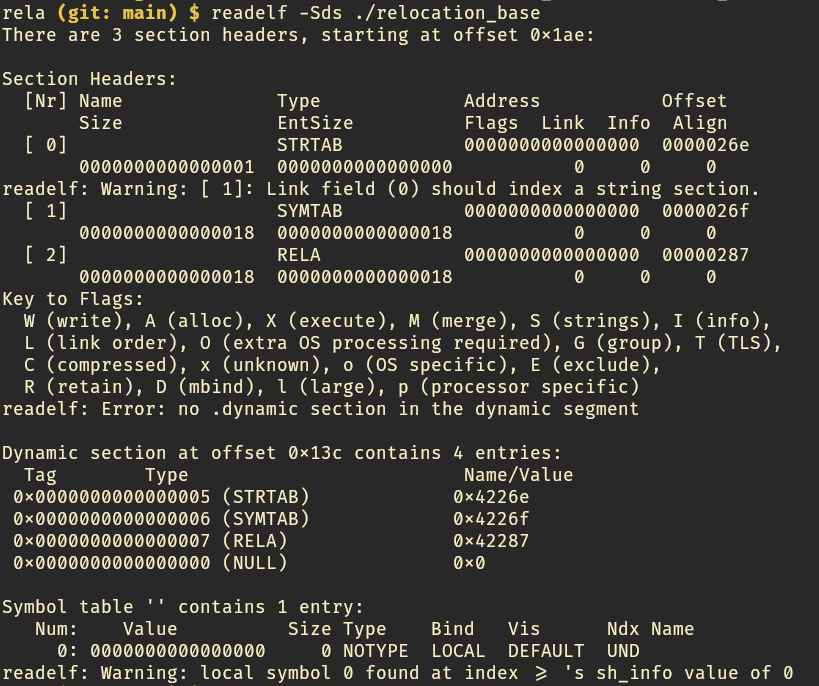
\includegraphics[width=\textwidth]{img/5-readelf.png}
\end{frame}

\begin{frame}[plain]
	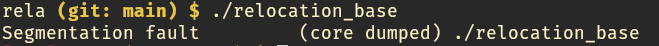
\includegraphics[width=\textwidth]{img/5-exec.png}
\end{frame}

\begin{frame}[plain]
	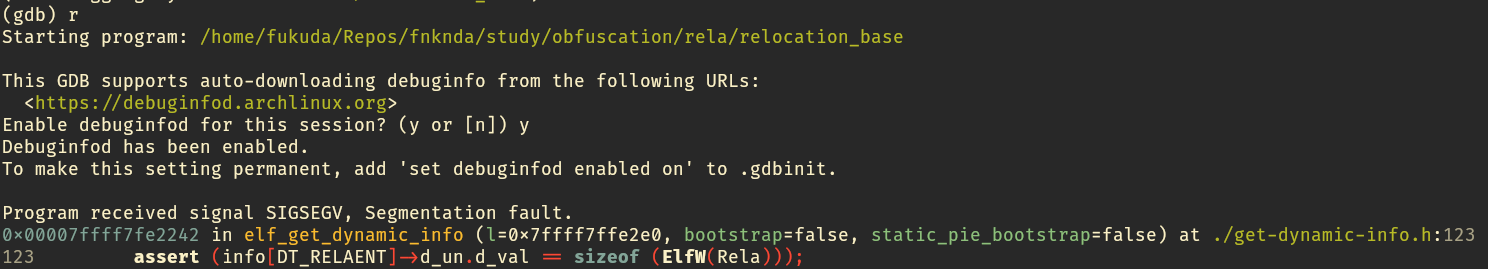
\includegraphics[width=\textwidth]{img/5-gdb.png}
\end{frame}

\begin{frame}[plain]
	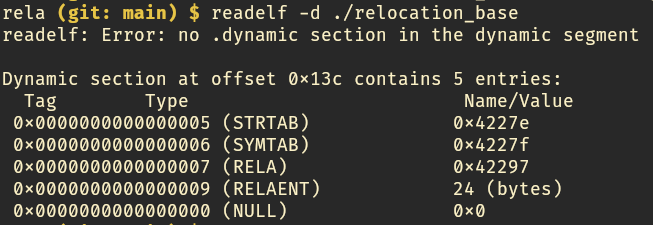
\includegraphics[width=\textwidth]{img/6-readelf.png}
\end{frame}

\begin{frame}[plain]
	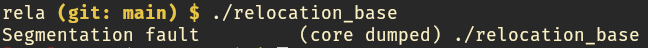
\includegraphics[width=\textwidth]{img/6-exec.png}
\end{frame}

\begin{frame}[plain]
	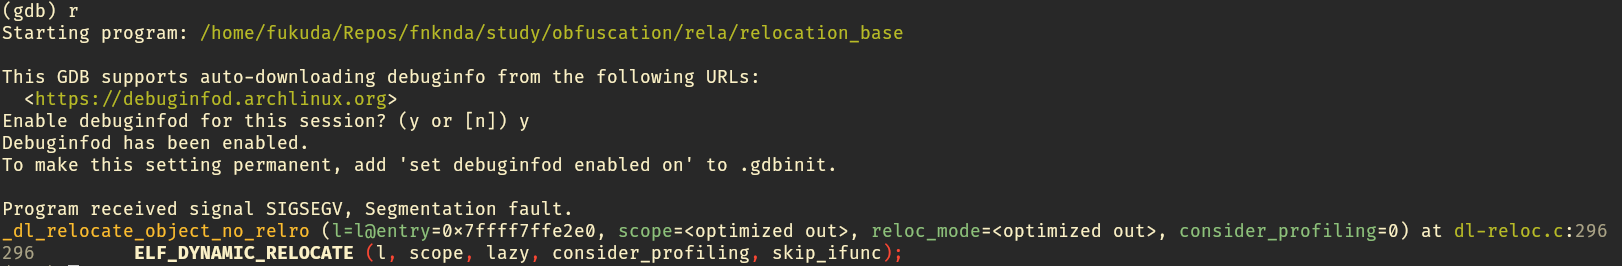
\includegraphics[width=\textwidth]{img/6-gdb.png}
\end{frame}

\begin{frame}[plain]
	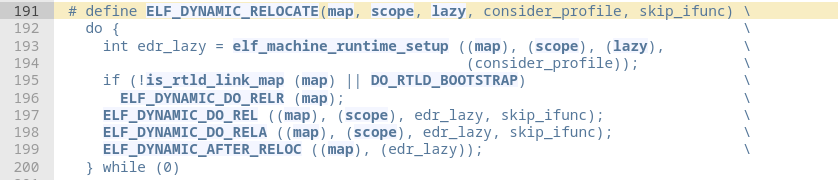
\includegraphics[width=\textwidth]{img/6-macro_source.png}
\end{frame}

\begin{frame}[plain]
	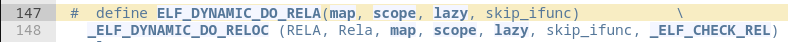
\includegraphics[width=\textwidth]{img/6-macro_follow_source.png}
\end{frame}

\begin{frame}[plain]
	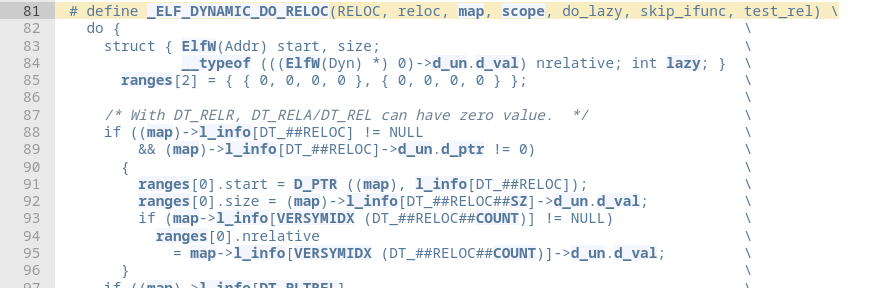
\includegraphics[width=\textwidth]{img/6-cause_source.png}
\end{frame}

\begin{frame}[plain]
	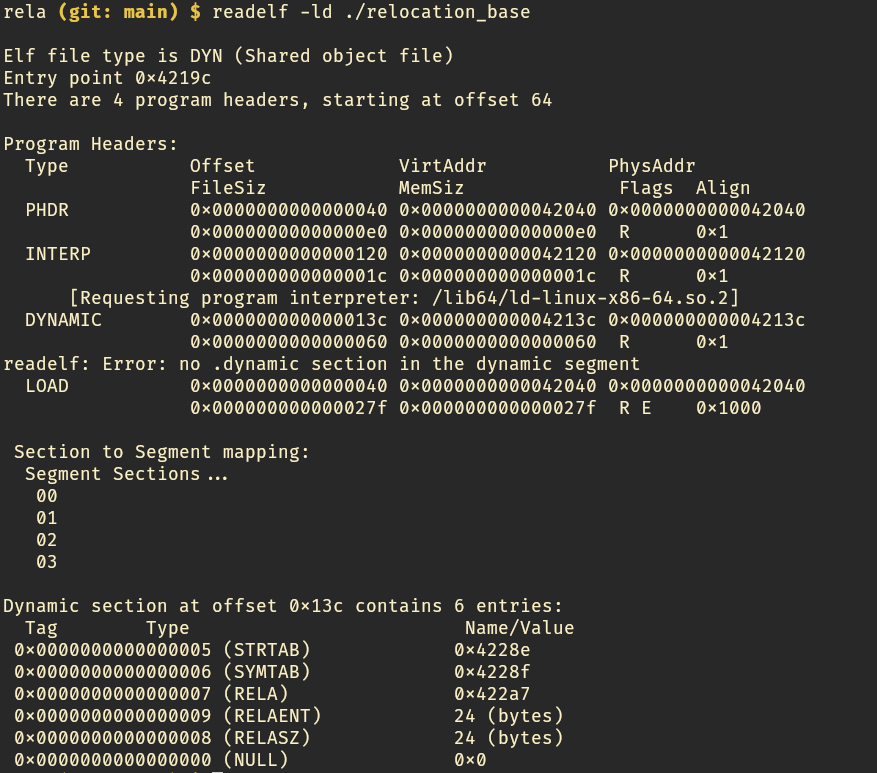
\includegraphics[height=\textheight]{img/7-readelf.png}
\end{frame}

\begin{frame}[plain]
	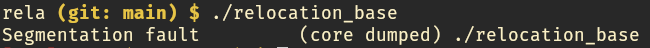
\includegraphics[width=\textwidth]{img/7-exec.png}
\end{frame}

\begin{frame}[plain]
	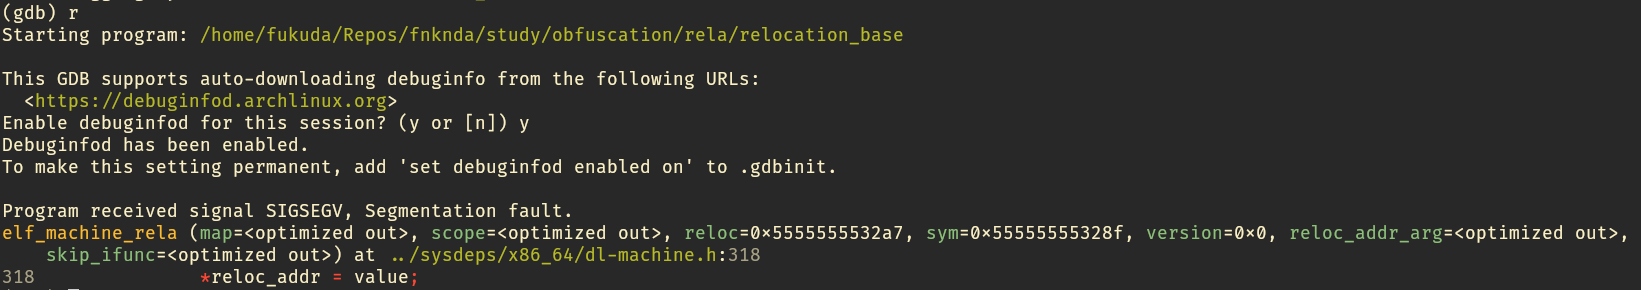
\includegraphics[width=\textwidth]{img/7-gdb.png}
\end{frame}

\begin{frame}
	\frametitle{Construindo do Zero}
	\framesubtitle{code}
	\begin{itemize}
		\item arrumar o \texttt{PT\_LOAD}
	\end{itemize}
\end{frame}

\begin{frame}[plain]
	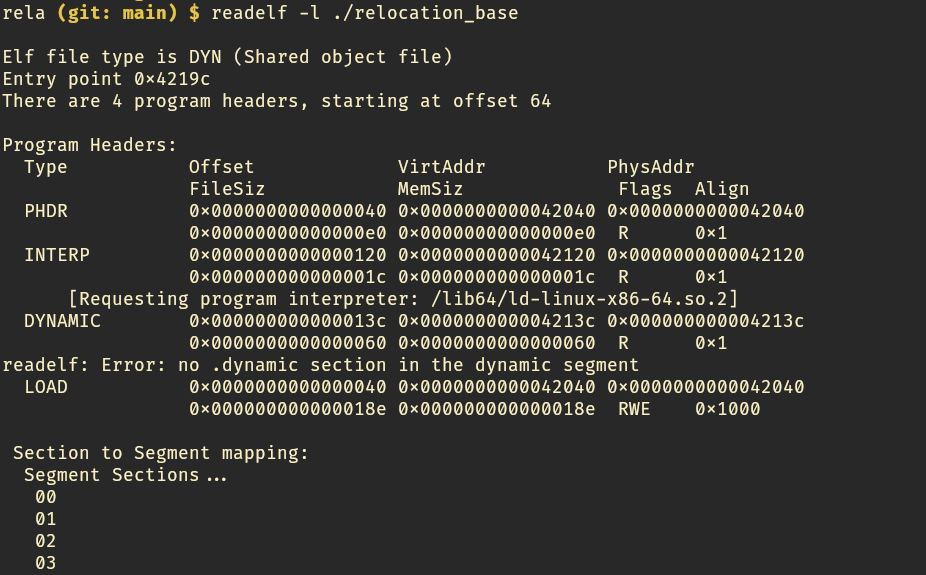
\includegraphics[width=\textwidth]{img/8-readelf.png}
\end{frame}

\begin{frame}[plain]
	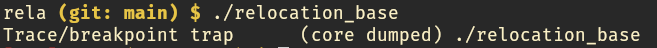
\includegraphics[width=\textwidth]{img/8-exec.png}
\end{frame}

\begin{frame}
	\frametitle{O Arquivo Final}
	\framesubtitle{file}
\end{frame}

\section{Resultados}

\begin{frame}
	\frametitle{Pontos Fortes}
	\framesubtitle{gdb}
	\begin{itemize}
		\item método incomum de ofuscação de entrypoint
		\item depende somente de ferramentas nativas
		\item logica de decoding externa e legitima
		\item dificulta análise dinâmica
	\end{itemize}
\end{frame}

\begin{frame}
	\frametitle{Pontos Fracos}
	\framesubtitle{gdb}
	\begin{itemize}
		\item permissão de mapeamento
		\item tipos de relocação
		\item espaço de relocação limitado
		\item muito trabalho para infectar um arquivo
	\end{itemize}
\end{frame}

\begin{frame}
	\frametitle{Detecção\cite{elf-rela-obfuscation}\cite{relobfuscate}}
	\framesubtitle{md5sum}
	\begin{itemize}
		\item mapas RWE
		\item alinhamento
		\item intersecções
		\item tipos de relocação
	\end{itemize}
\end{frame}

\begin{frame}[allowframebreaks]
	\frametitle{Referências}
	\framesubtitle{ldd}
	\printbibliography[heading=none]
\end{frame}

\section{Perguntas?}

\begin{frame}
	\frametitle{Fim}
	\framesubtitle{exit}
	Muito obrigado :):
\end{frame}

\end{document}
